% To compile single chapters put a % symbol in front of "\comment" and "}%end of comment" below 
%    and take off the % symbol from "\end{document" at the bottom line. Undo before compiling
%    the complete thesis
%%Note: You can only use \section command, you are not allowed, per TTU Graduate School, use
%%\subsection command for ghigher level subheadings. At most level 2 subheadings are allowed.

\chapter{DASP Algorithm Development}
\label{DASP Algorithm Development Chapter}

\section[DASP Overview]{DASP Overview}

The processing of conducted URE for the purposes of device classification often requires intimate knowledge of the underlying signal characteristics which are determined by the physical implementation of the device's electronic circuitry.  DASP provides a method for aligning those signal dimensions inherent to the majority of electronic circuits without prior knowledge of the device's physical or conducted noise characteristics.  The following DASP algorithms are presented to align conducted URE dimensions of interest for device classification: Harmonically Aligned Signal Projection (HASP), Modulation Aligned Signal Projection (MASP), Cross-Modulation Aligned Signal Projection (CMASP), and Spectral Correlation Aligned Projections (SCAP).   In addition, two different methods for implementing the HASP algorithm will be presented, the fixed and decimating types.

An additional DASP algorithm widely used within the signal processing community is the Short-Time Fourier Transform (STFT, sometimes referred to as a spectrogram) \cite{Welch1967, Allen1977, Griffin1984}.  The STFT computes the Fast Fourier Transforms (FFT) over short time segments and \textit{aligns} the frequency bins of these FFT segments over time.  For consistency, I will use the term Frequency Aligned Signal Projection (FASP) for the STFT when used in the context of a DASP transform.   

Techniques for processing and extracting features from DASP output arrays are discussed in Chapter \ref{DASP Feature Extraction Chapter}.  Chapter \ref{DASP Device Classification Chapter} provides results from the application of supervised and unsupervised machine learning techniques to DASP generated arrays and features to determine the applicability of dimensional alignments to classify devices based upon their URE.

\section[Harmonically Aligned Signal Projection (HASP)]{Harmonically Aligned Signal Projection}
\label{Harmonically Aligned Signal Projection}

The HASP algorithm provides a method for aligning a fundamental frequency with its respective harmonics in the column of a 2D matrix.   Harmonic content analysis can provide information related to a signal's stability, shape, and the underlying physical circuitry.  All non-pure sinusoidal periodic functions, such as square or triangle waves, are composed of harmonics with varying magnitudes and phases which define the shape of the time domain signal.  Aligning the harmonic structure of a signal is complicated by frequency uncertainties and offsets of the underlying fundamental.  For instance, the $40$th harmonic of a $50$Hz signal should be at $2000$Hz exactly, however a $0.5$Hz offset in the fundamental will result in the $40$th harmonic appearing at $2020$Hz.  Assuming a $1$Hz frequency resolution in the FFT, the harmonic will appear $20$ bins from where expected. To demonstrate, Figure \ref{fig:harm_aligned_example} shows the alignment of frequency bins through the $40$th harmonic for an exact $50$Hz signal and one with a $0.5$Hz offset. 

\begin{figure}[tb]
	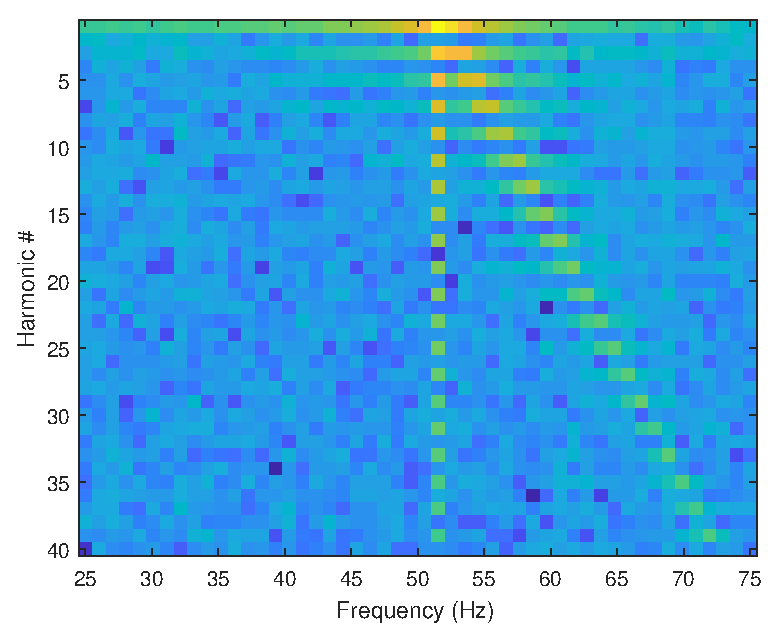
\includegraphics[width=\textwidth]{./dasp_algorithm_results/harmonic_aligned_example.eps}
	\centering
	\caption{Image showing the alignment of the harmonics of $50$Hz and $50.5$Hz square waves from a synthetic test signal generated from the addition of two square waves with $50$Hz and $50.5$Hz fundamental frequencies.  The frequency of each row is multiplied by the harmonic number, such that the center bin of the second row is $2 \times 50$Hz$ = 100$Hz.  The last row shows the $40$th harmonic of the $50$Hz signal at $2000$Hz and the $40$th harmonic of the $50.5$Hz signal at $2020$Hz.}
	\label{fig:harm_aligned_example}
\end{figure}

In addition to the misalignment of the $50.5$Hz fundamental with its respective harmonics, the harmonic structure of a square wave is evidenced by the alternating intensities of harmonics.  Every odd harmonic row (i.e. $3$rd, $5$th, $7$th, etc.) shows a harmonic signal, whereas the even harmonic rows ($2$nd, $4$th, $6$th, etc.) do not appear to show any harmonic structure.

\subsection[Harmonically Aligned Signal Projection - Fixed Type (HASP-F)]{Harmonically Aligned Signal Projection - Fixed Type (HASP-F)}
\label{Harmonically Aligned Signal Projection - Fixed Type}

Figure \ref{fig:harm_aligned_example} provides an example of the Fixed Type HASP algorithm (HASP-F), where a fixed number of frequency bins are selected around a specific fundamental and its respective harmonics and are aligned in to rows to form a 2-D image.  Assuming the fundamental frequency is known perfectly, the harmonics will align within a single column and provide a strong feature that could be used for classification purposes, as shown in the diagram of the HASP-F process in Figure \ref{fig:haspf_diagram_independent}.  In addition, modulation sidebands centered around the fundamental frequency and its harmonics also align within the HASP-F image, as shown in Figure \ref{fig:haspf_diagram_modulation}, and provide an additional dimension alignment and further insights in to the underlying signal structure.

\begin{figure}[tb]
	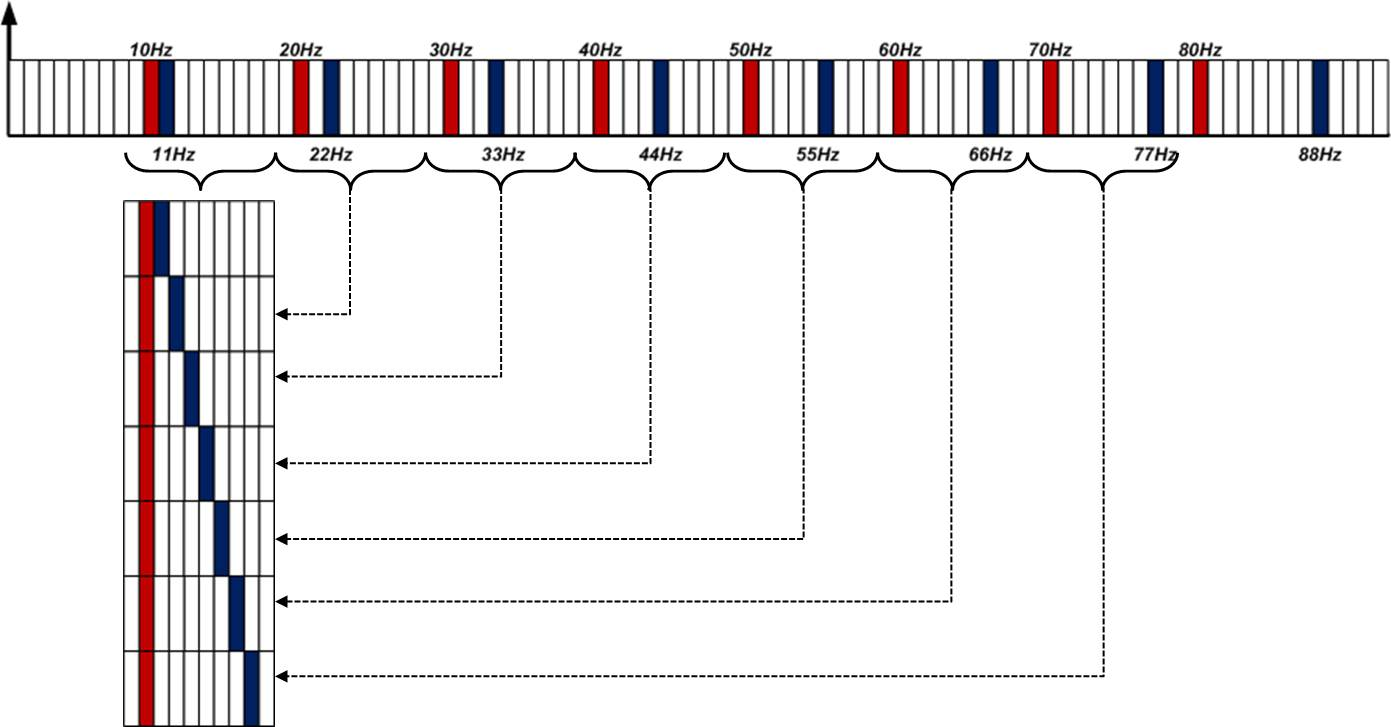
\includegraphics[width=\textwidth]{./misc_graphics/haspf_diagram_independent.jpg}
	\centering
	\caption{Diagram of the HASP-F process applied to two independent carriers at $10$Hz and $11$Hz with harmonic content, as represented by the red and blue blocks, respectively, and each frequency bin represents a $1$Hz resolution.  As a fixed number of bins are selected to align the $10$Hz harmonics, the $11$Hz harmonics slant across the image.}
	\label{fig:haspf_diagram_independent}
\end{figure}

\begin{figure}[tb]
	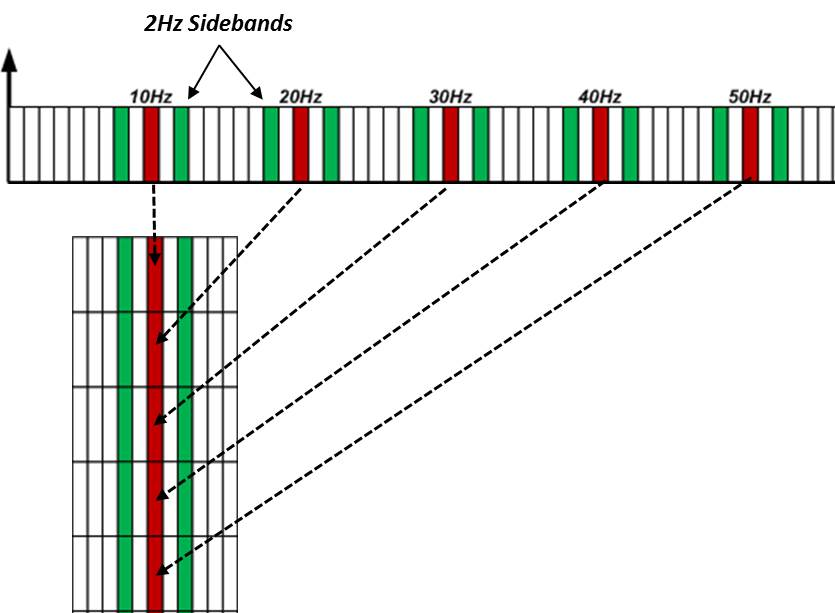
\includegraphics[width=\textwidth]{./misc_graphics/haspf_diagram_modulation.jpg}
	\centering
	\caption{Diagram of the HASP-F process applied to a carrier at $10$Hz with $2$Hz modulation sidebands, as represented by the red and green blocks, respectively.  As a fixed number of bins are selected to align the $10$Hz harmonics, the $2$Hz sidebands also align accordingly.}
	\label{fig:haspf_diagram_modulation}
\end{figure}

As demonstrated in Figure \ref{fig:haspf_diagram_independent}, the $10$Hz fundamental frequency aligns with its respective harmonics when a fixed number of frequency bins are selected around each harmonic, whereas, the $11$Hz independent carrier slants across the 2-D array because each progressive $11$Hz harmonic is $1$Hz, or $1$ frequency bin, further away from the corresponding $10$Hz harmonic.  Because modulation sidebands are always at fixed frequencies around both the fundamental and its harmonics, Figure \ref{fig:haspf_diagram_modulation} shows that modulation sidebands also align when performing fixed harmonic alignment. 

As evidenced from Figure \ref{fig:haspf_diagram_independent} and Figure \ref{fig:haspf_diagram_modulation}, the fixed harmonic alignment requires a specific fundamental frequency to be known and selected for perfect vertical alignment to occur, otherwise any frequency offset will result in a slanted line in the resulting 2-D image.  The HASP-F algorithm is described in more detail in Algorithm \ref{alg:haspfalg}. The algorithm operates on a frequency domain input, $\hat{r}$, along with the input parameters $f_c$ and $B$, center frequency and bandwidth, respectively. The final 2D image will be a function of $f_c$, the center frequency of the image, and $B$, the bandwidth around this center frequency (or width of the image). The algorithm first derives the maximum harmonic, $K$, of $f_c$, based on the sampling frequency and the bandwidth around $f_c$.  The maximum harmonic, $K$, corresponds to the height of the 2-D HASP image, where each row of the image corresponds to the $k$th harmonic of $f_c$. The image is formed by iterating through all harmonics from the fundamental frequency to the maximum harmonic $K$.  For each harmonic, the magnitude of the input PSD, $\hat{r}$, is indexed by the corresponding $(k \times f_c) \pm B$ frequency bins, where $k$ is the harmonic number $\left[1,2,3 \ldots{} K \right]$.  Each row is comprised of a fixed number of frequency bins as set by the bandwidth, $B$, around the fundamental frequency.  The resulting HASP-F image dimensions are $K$ by the number of discrete frequency bins comprising the continuous frequencies $f_c \pm B$. 
 
\begin{algorithm}
	\caption{Harmonic Aligned Signal Projection Algorithm - Fixed Type (HASP-F)} \label{alg:haspfalg}
	\scriptsize
	\centering
	\begin{algorithmic}[1]
		\Require~~
		\Statex $\hat{r}$ - Input Power Spectrum
		\Statex $f_c$ - Center Frequency 
		\Statex $B$ - Bandwidth
		\Ensure~~
		\Statex $\bf{H}$ - HASP Output Array
		\Statex
		\For  {$k = 1, 2, \ldots K$} 
		\State    $\mathbf{f}_k \gets \left[ \hat{r}(x_i) \right], (k \times f_c) - B \leq x_i \leq (k \times f_c) + B$
		\State		$k$-th row of $\mathbf{H} \gets \mathbf{f}_k$
		\EndFor
	\end{algorithmic}
\end{algorithm}

To illustrate the HASP-F algorithm images, conducted URE was collected from fluorescent lights in an RF shielded enclosure using a USRP N210 collection platform with an LFRX analog to digital processing board operating at $2$MS/s, as described in Chapter \ref{URE Data Collection Chapter}.  Figure \ref{fig:hasp_fft_example} is a plot of the FFT of the conducted URE collected from two fluorescent light fixtures, showing a fundamental frequency at approximately $45$kHz along with $21$ harmonics up to $1$MHz.  Figure \ref{fig:haspf_example} is the resulting image after application of the HASP-F algorithm to the frequency spectrum of the same time-domain capture.  The blurred vertical line and additional blurred slanting line represent the harmonic structure of the two different fluorescent lights with a very minute frequency difference between their respective crystal oscillators.  The center frequency, $f_c$, of the HASP-F image was selected to vertically align one of the oscillators resulting in a progressively increasing offset for each harmonic of the second crystal oscillator.  

\begin{figure}[tp]
	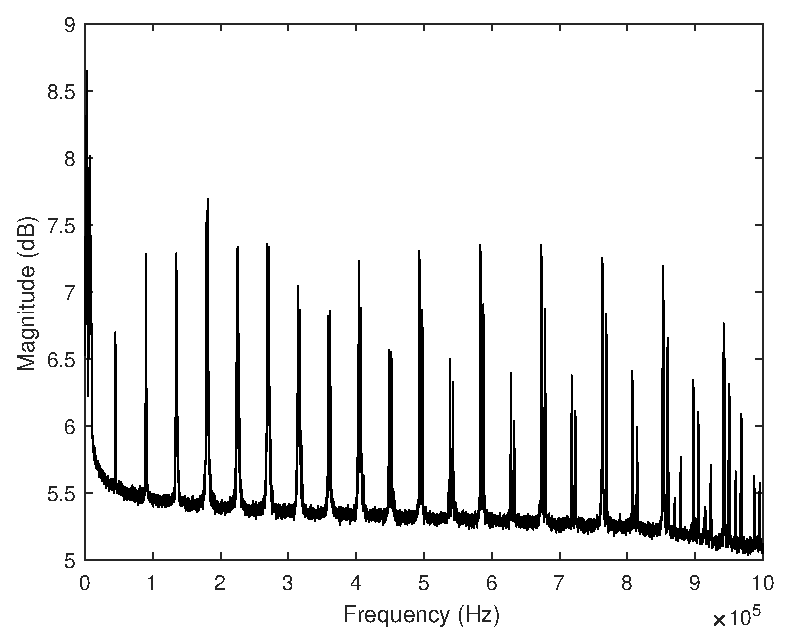
\includegraphics[width=\textwidth]{./dasp_algorithm_results/hasp_fft_filenum_9601.eps}
	\centering
	\caption{Plot of an FFT derived from a time domain capture of conducted URE from a set of fluorescent lights.  The lights have a dominant URE signal with an approximate $45$kHz fundamental frequency.  The plot shows the slight separation of the URE from the two lights at higher frequencies due to the minor differences in the electronic ballasts used within the different lights.}
	\label{fig:hasp_fft_example}
\end{figure}

\begin{figure}[tp]
	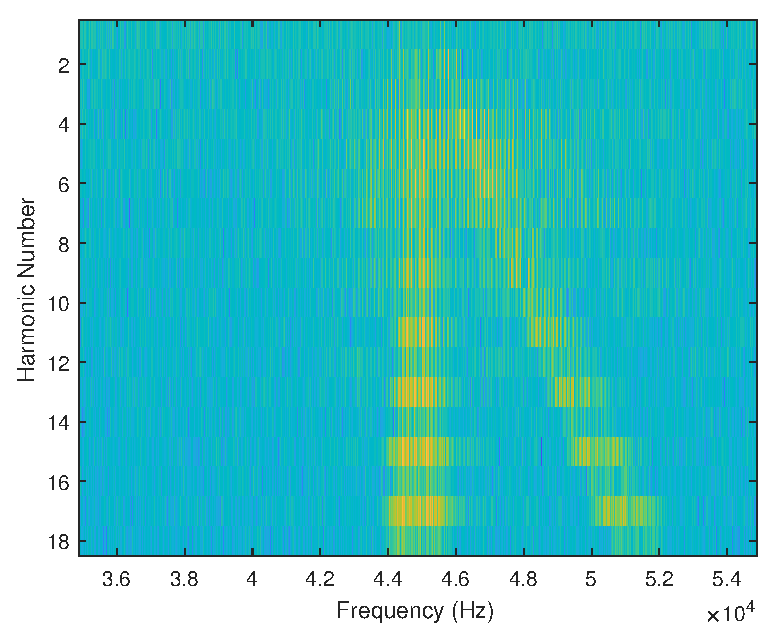
\includegraphics[width=\textwidth]{./dasp_algorithm_results/hasp_f_wide_filenum_9601.eps}
	\centering
	\caption{HASP-F output of the frequency domain signal shown in \ref{fig:hasp_fft_example}.  The separation of harmonics at higher frequencies for the two electronic ballasts can be seen, however the two harmonic alignments are blurred which further demonstrate a low level modulation or instability in the fundamental frequency of the URE generators.}
	\label{fig:haspf_example}
\end{figure}

Analysis of Figure \ref{fig:haspf_example} shows that the two URE generators were roughly $7$kHz apart at the $18$th harmonic.  The frequency offset between the oscillators in the two fluorescent lights was then approximated to be $390$Hz by $7$kHz $/18 \approx 390$Hz.  

\subsection[Harmonically Aligned Signal Projection - Decimation Type (HASP-D)]{Harmonically Aligned Signal Projection - Decimation Type (HASP-D)}
\label{Harmonically Aligned Signal Projection - Decimation Type}

Although the HASP-F algorithm provides a method for aligning harmonics and modulation sidebands, the fundamental frequency needs to be known precisely or the fundamental frequency harmonics will not vertically align and, in addition, the harmonic structures of independent carriers within the HASP-F image will form a slanted line.  The HASP Decimation type (HASP-D) algorithm was developed to vertically align the harmonics of independent signals regardless of the chosen center frequency or amount of frequency offset between the carriers.  The HASP-D algorithm is illustrated in Figure \ref{fig:haspd_diagram_independent}, where each progressive harmonic row is decimated to a fixed number of bins to realign independent harmonics.  Although independent carriers and their respective harmonics align vertically, modulation sidebands ``curve'' in toward the aligned harmonics as the bandwidth around the fundamental is collapsed in to fewer and fewer bins through the decimation process, as shown in Figure \ref{fig:haspd_diagram_modulation}.

\begin{figure}[tp]
	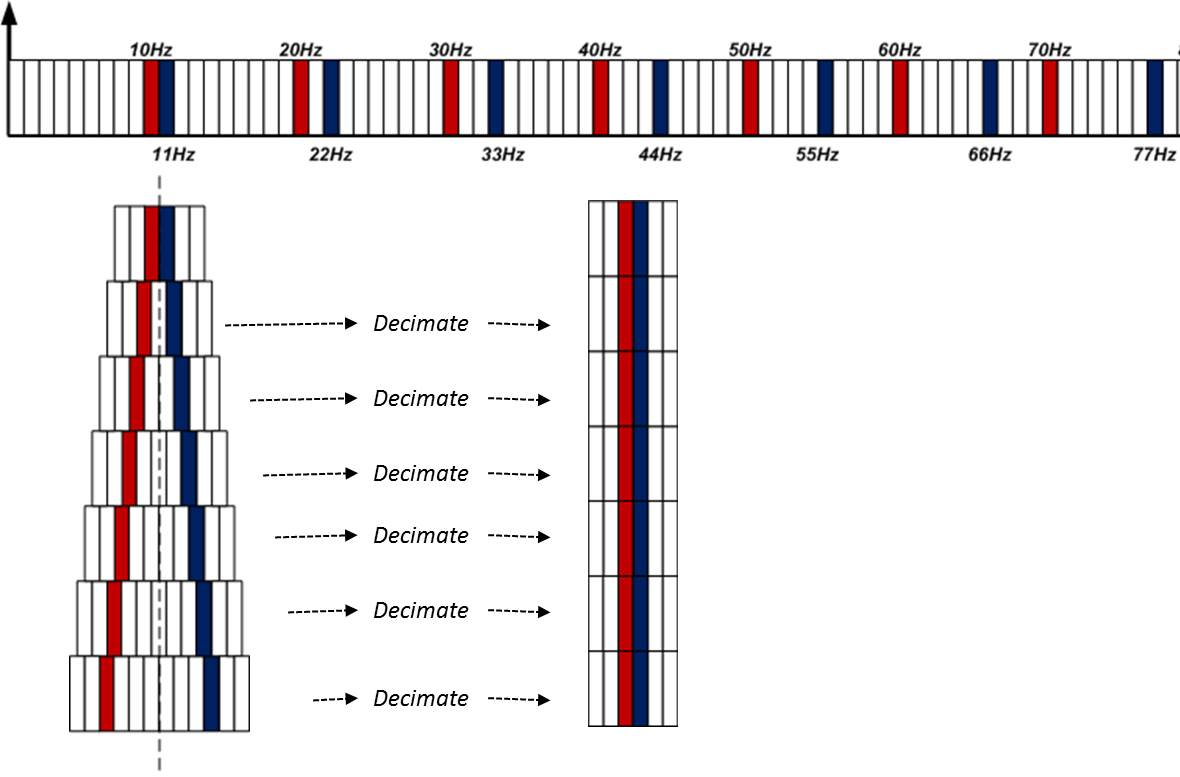
\includegraphics[width=\textwidth]{./misc_graphics/haspd_diagram_independent.jpg}
	\centering
	\caption{Diagram of the HASP-D process applied to a two independent carriers at $10$Hz and $11$Hz with harmonic content, as represented by the red and blue blocks, respectively.  As each harmonic row is added, the number of bins is decimated to equal the number of bins around the fundamental, thus aligning the independent carriers.}
	\label{fig:haspd_diagram_independent}
\end{figure}

\begin{figure}[tp]
	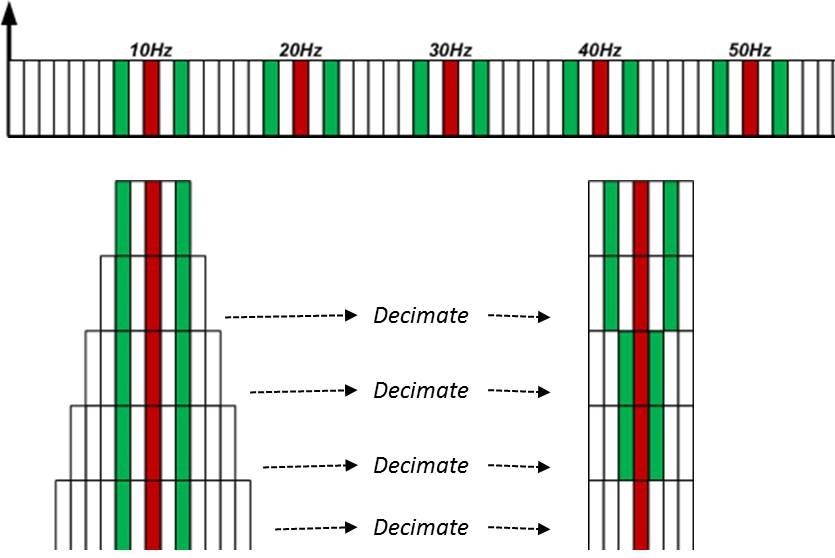
\includegraphics[width=\textwidth]{./misc_graphics/haspd_diagram_modulation.jpg}
	\centering
	\caption{Diagram of the HASP-D process applied to a carrier at $10$Hz with $2$Hz modulation sidebands, as represented by the red and green blocks, respectively.  As each harmonic row is added, the number of bins is decimated to equal the number of bins around the fundamental, thus causing the modulation sidebands to curve in to eventually add with the carrier frequency harmonics.}
	\label{fig:haspd_diagram_modulation}
\end{figure}

As shown in Figure \ref{fig:haspd_diagram_independent}, the number of bins selected around the fundamental frequency determines the resulting number of bins for each harmonic row.   With each progressive harmonic, the number of indexed bins expands by the harmonic number and is then subsequently decimated by the corresponding harmonic number resulting in a vector of bins corresponding to the number of bins in the fundamental frequency row.   By collapsing each row through the decimation process, independent carriers align with their respective harmonics, whereas modulation sidebands that are a fixed number of bins around a given harmonic are ``squeezed'' in toward their respective carrier frequency.   

The HASP-D algorithm is described in more detail in Algorithm \ref{alg:haspdalg} and only differs slightly from the HASP-F algorithm. Identical to the HASP-F algorithm, the HASP-D algorithm operates on a frequency domain input, $\hat{r}$, and requires center frequency and bandwidth input parameters, $f_c$ and $B$, respectively.  The algorithm derives the maximum harmonic, $K$, of $f_c$, based on the sampling frequency and the bandwidth around $f_c$. The maximum harmonic, $K$, corresponds to the height of the 2-D HASP image, where each row of the image corresponds to the $k$th harmonic of $f_c$. The image itself is created by iterating through all harmonics from the fundamental frequency to the maximum harmonic $K$.  For each harmonic, the $\hat{r}$ vector is indexed by the corresponding $k(f_c \pm B)$ frequency bins, where $k$ is the harmonic number $\left[1,2,3 \ldots{} K \right]$.  Because of the expansion of each harmonic vector at increasing $k$, each vector is downsampled by a factor of $k$ to align harmonically related bins in the HASP-D image.  The resulting HASP-D image dimensions are $K$ by the number of discrete frequency bins comprising the continuous frequencies $f_c \pm B$, which are the same dimensions as the HASP-F image.

\begin{algorithm}
	\caption{Harmonic Aligned Signal Projection Algorithm - Decimation Type (HASP-D)} \label{alg:haspdalg}
	\scriptsize
	\begin{algorithmic}[1]
		\Require~~
		\Statex $\hat{r}$ - Input Power Spectrum
		\Statex $f_c$ - Center Frequency 
		\Statex $B$ - Bandwidth
		\Ensure~~
		\Statex $\bf{H}$ - HASP-D Output Array
		\Statex
		\For  {$k = 1, 2, \ldots K$} 
		\State    $\mathbf{f}_k \gets \left[ \hat{r}(x_i) \right], k(f_c - B) \leq x_i \leq k(f_c + B)$
		\State		$k$-th row of $\mathbf{H} \gets$ DOWNSAMPLE $\mathbf{f}_k$ by factor of $k$
		\EndFor
	\end{algorithmic}
\end{algorithm}

To further analyze the URE signal processed by the HASP-F algorithm in Figure \ref{fig:haspf_example}, the HASP-D algorithm was applied to the same frequency domain signal, as shown in Figure \ref{fig:haspd_example}.  The HASP-D image demonstrates the alignment of independent fundamental frequencies and their respective harmonics.  The two vertical lines centered around $45$kHz represent the two independent oscillator signals previously identified in Figure \ref{fig:hasp_fft_example} and Figure \ref{fig:haspf_example}.  The frequency offset between the two oscillators was found to be approximately $300$Hz through visual inspection which roughly corresponds to the calculations derived from the HASP-F image in Figure \ref{fig:haspf_example}.

\begin{figure}[tp]
	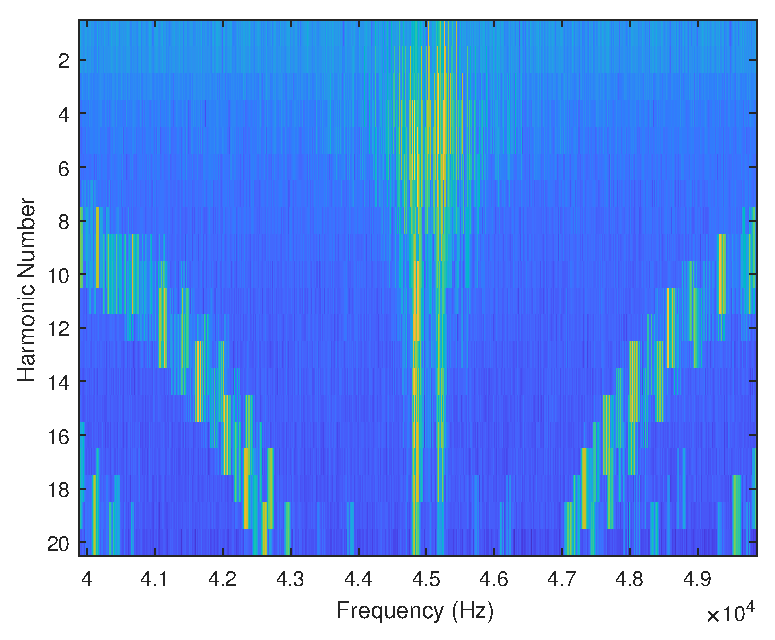
\includegraphics[width=\textwidth]{./dasp_algorithm_results/hasp_d_filenum_9601.eps}
	\centering
	\caption{HASP-D output of the frequency domain signal shown in Figure \ref{fig:hasp_fft_example}.  The HASP-D algorithm decimates each progressive harmonic row to realign harmonic frequency bins to the fundamental frequency row (i.e. row number $1$).  The two independent URE generator signals are now fully parallel because their respective harmonics are aligned across each harmonic row through the decimation process.}
	\label{fig:haspd_example}
\end{figure}

The curved lines centered on the independent carriers in Figure \ref{fig:haspd_example} are artifacts of the preceding and following carrier harmonics due to the expansion and subsequent decimation of each increasing harmonic row.  This was verified by calculating the frequency difference between the curved lines and the harmonic frequency at the $20$th harmonic row, $20 \times (44.8 - 42.6)$kHz $\approx 45$kHz, which corresponds to the fundamental frequency as well as the frequency spacing between all harmonics.

As previously noted in Figure \ref{fig:haspf_example}, the HASP-F image shows a blurring of the two independent carriers which were examined further by applying the HASP-D algorithm with a smaller bandwidth as shown in Figure \ref{fig:haspd_example_zoom}. The blurring, or instability, in Figure \ref{fig:haspf_example} appeared to be the result of a moderate oscillator instability and a low level modulation of the URE generator carrier frequency, as illustrated by the width of the center aligned harmonics and the curved modulation lines, respectively.  

\begin{figure}[tp]
	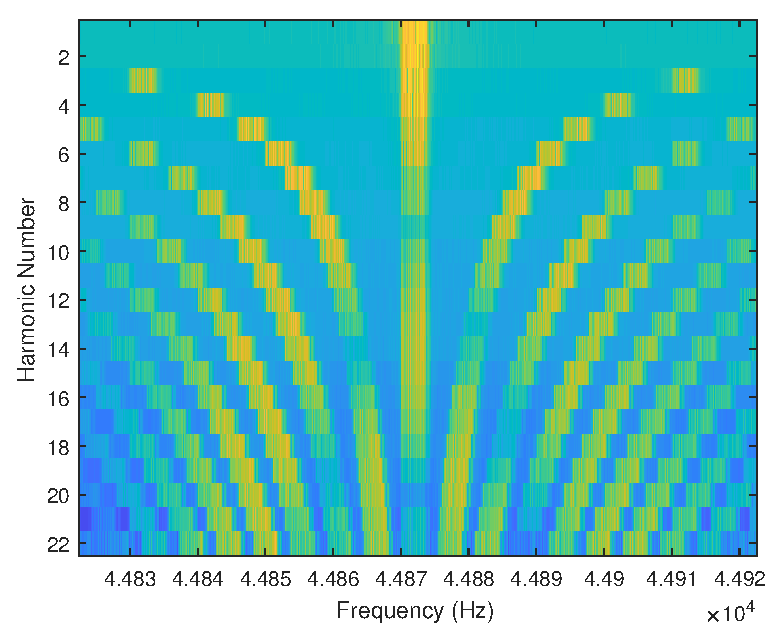
\includegraphics[width=\textwidth]{./dasp_algorithm_results/hasp_d_zoom_filenum_9601.eps}
	\centering
	\caption{Zoomed in view of the HASP-D output of the frequency domain signal shown in Figure \ref{fig:hasp_fft_example}.  The blurring was found to be approximately $4$Hz wide resulting in roughly $\pm 45$ppm carrier stability.  The curved lines centered around the carrier frequency were due to $120$Hz modulations of the carrier frequency.}
	\label{fig:haspd_example_zoom}
\end{figure}

The oscillator instability was found to be approximately $4$Hz wide, corresponding to an approximate clock stability of $\pm 45$ppm, which is consistent with typical inexpensive crystal oscillators.  The sideband peak frequency offsets were found to be approximately $120$Hz, or the second harmonic of the $60$Hz power line frequency, by examining the $3$rd harmonic of the carrier frequency, $3 \times (4.4872\times10^4 - 4.4832\times10^4)$Hz$ = 120$Hz, indicating a $120$Hz power line harmonic frequency amplitude modulation of the fluorescent light oscillators.

An additional HASP alignment method, HASP Interpolating type (HASP-I), is described further in Appendix A.  The HASP-I algorithm operates in much the same way as the HASP-D algorithm, except that it utilizes an interpolation method for realigning independent carrier frequency harmonics as opposed to the decimation process used with HASP-D.  The HASP-I algorithm was not evaluated further because of processing time constraints and redundancy with the HASP-D algorithm, but is presented for completeness.    

\section[Modulation Aligned Signal Projection (MASP)]{Modulation Aligned Signal Projection (MASP)}
\label{Modulation Aligned Signal Projection}

The MASP algorithm provides a method for characterizing amplitude modulations (AM) in URE time domain signal captures without assumptions of the underlying carrier or modulation frequencies.  The MASP algorithm operates on a time domain signal by first applying a STFT and then performing an FFT across all time slices for each frequency column.  The resulting 2-D structure is a frequency-by-frequency matrix where the vertical axis represents the modulation frequencies and the horizontal axis represents the carrier frequencies. Whereas HASP aligns harmonically related frequencies within a URE signal, MASP aligns modulation and carrier frequencies by calculating and highlighting their respective intersections.

MASP is described in depth in Algorithm \ref{alg:maspalg}. MASP operates on a time domain input signal, $r$, by first performing a STFT with no overlap on the captured URE signal.  The sample rate, collection time, and maximum modulation frequency of interest, $f_m$, dictate the length of the time slices within the STFT and hence the pixel resolution of the resulting MASP output image.  As $f_m$ is increased, shorter time slices are utilized by the STFT resulting in a decreased number of frequency bins in the carrier frequency, $f_c$, columns.  The total collection time of $r$ determines the resolution of the $f_m$ rows and the sample rate of $r$ determines the maximum carrier frequency.  Once the magnitude of the STFT transform, $\bf{S}$, is calculated, the algorithm iterates through all carrier frequency bins, $k$, and performs an FFT on each frequency column.  The magnitude of the frequency column FFTs then form a column within the MASP image.  The resulting MASP image is a frequency-by-frequency matrix where rows represent modulation frequencies and columns represent carrier frequencies.  A peak in the MASP image provides a visual indication of a significant amplitude modulation at a specific modulation and carrier frequency.

\begin{algorithm}
	\caption{Modulation Aligned Signal Projection Algorithm (MASP)} \label{alg:maspalg}
	\scriptsize
	\begin{algorithmic}[1]
		\Require~~
		\Statex $r$ - Input Time Domain Signal
		\Statex $N$ - Number of Time Slices for Short-Time Fourier Transform
		\Ensure~~
		\Statex $\mathbf{M}$ - MASP Output Array
		\Statex
		\State $\mathbf{S} \gets $ Short-Time Fourier Transform of $r$ over $N$ non-overlapping time slices
		\State $\mathbf{S} \gets \left|\bf{S}\right|$ 
		\ForAll  {$k$} 
		\State      $\mathbf{S}_k \gets k$-th column of $\mathbf{S}$
		\State		$\mathbf{T}_k \gets $ FAST FOURIER TRANSFORM of $\mathbf{S}_k$
		\State		$k$-th column of $\mathbf{M} \gets \left|\mathbf{T}_k\right|$
		\EndFor
	\end{algorithmic}
\end{algorithm}

Figure \ref{fig:masp_example} shows the MASP output image as applied to the conducted URE spectrum demonstrated in Figures \ref{fig:hasp_fft_example}, \ref{fig:haspf_example}, and \ref{fig:haspd_example}. The MASP image shows that the device under test has a strong harmonic structure with an approximately $45$kHz fundamental frequency; however, unlike with HASP, MASP was also able to extract a strong, but low frequency, modulating frequency around $20$Hz along with the harmonics of $20$Hz. Such a structure is often buried in and confounded by the stronger fundamental frequencies and their respective harmonics which further supports the utilization of dimensional alignments for feature extraction.  Additionally, the amplitude modulation index can be very low with the modulation sidebands around the carrier frequency near the noise floor, further obfuscating amplitude modulation features.

\begin{figure}[tp]
	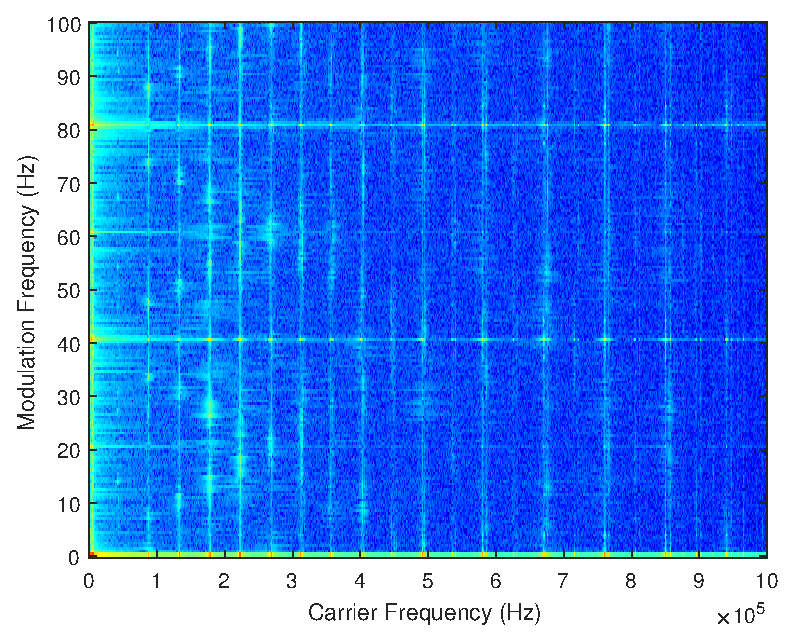
\includegraphics[width=\textwidth]{./dasp_algorithm_results/masp_low_filenum_9601.eps}
	\centering
	\caption{MASP output image derived from the time domain capture of the URE in Figure \ref{fig:hasp_fft_example}.  The vertical lines represent potential carriers across the entire capture spectrum and the horizontal lines represent amplitude modulations across the entire spectrum.  The intersection of these lines represents the location of a modulated carrier.  In addition to the strong frequency peaks identified in Figure \ref{fig:hasp_fft_example}, modulations frequencies can be found at $20$Hz and its respective harmonics.}
	\label{fig:masp_example}
\end{figure}

In addition to the modulations occurring at $20$Hz and its harmonics, several unrelated modulation and carrier frequency intersections were identified in Figure \ref{fig:masp_example}.  For instance, significant peaks were identified at the intersection of the fourth harmonic of the dominant carrier frequency, approximately $180$kHz, and modulations frequencies of $15$Hz and $25$Hz, indicating a strong amplitude modulation which was not identified during analysis of the HASP-F and HASP-D images.

\section[Spectral Correlation Aligned Projection (SCAP)]{Spectral Correlation Aligned Projection (SCAP)}
\label{Spectral Correlation Aligned Projection}

The SCAP algorithm provides a method for aligning frequency spacings between peaks in the frequency domain.  Fixed frequency spacings can result from frequency harmonics, frequency mixing, or frequency and amplitude modulations; and furthermore, can occur at multiple unrelated locations within the conducted URE spectrum. The SCAP algorithm provides two outputs, $\bf{S}_H$ and $\bf{S}_F$, where $\bf{S}_F$ is the autocovariance, $\bf{C}_{XX}$, of $\hat{r}$ and $\bf{S}_H$ results from the application of the HASP-D algorithm to $\bf{S}_F$, as described in Algorithm \ref{alg:scapalg}. 

\begin{algorithm}
	\caption{Spectral Correlation Aligned Projection Algorithm} \label{alg:scapalg}
	\scriptsize
	\begin{algorithmic}[1]
		\Require~~
		\Statex $\hat{r}$ - Input Power Spectrum
		\Ensure~~
		\Statex $\bf{S}_H$ - SCAP Output
		\Statex $\bf{S}_F$ - Spectral Autocovariance Vector 
		\Statex
		\State $\bf{S}_F \gets \bf{C}_{XX}(\hat{r})$
		\State $\bf{S}_H \gets $ HASP-D of $\bf{S}_F$ 
	\end{algorithmic}
\end{algorithm}

Figure \ref{fig:scap_xcov_example} shows the autocovariance of $\hat{r}$, $\bf{S}_F$, of the conducted URE spectrum illustrated in Figure \ref{fig:hasp_fft_example}, with $\bf{S}_H$ shown in Figure \ref{fig:scap_hasp_example} after application of the HASP-D algorithm.  The HASP-D algorithm was configured with $f_c = 1000$Hz and $B = 1900$Hz and a maximum harmonic of $K = 10$.  In addition, $\bf{S}_F$ was scaled such that the maximum peak value equals one and the frequency correlation axis was limited from $100$kHz to $70$Hz with a reverse semi-log scale.

\begin{figure}[tp]
	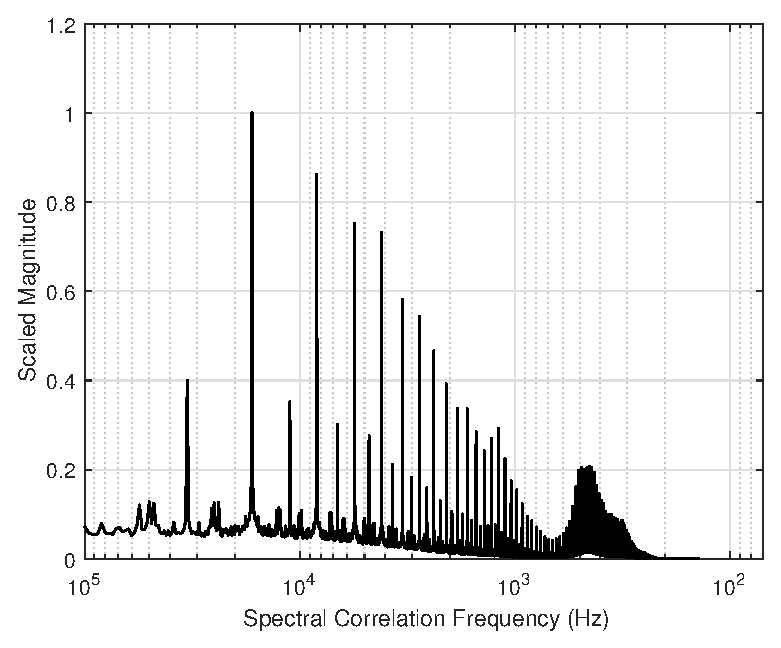
\includegraphics[width=\textwidth]{./dasp_algorithm_results/scap_filenum_12001.eps}
	\centering
	\caption{Plot of the autocovariance of the FFT shown in Figure \ref{fig:hasp_fft_example}.  The peaks within the plot represent the correlation of equally spaced frequency peaks within the FFT, with a dominant correlation at $16.67$kHz, which corresponds to roughly $120$ FFT bins.}
	\label{fig:scap_xcov_example}
\end{figure}

\begin{figure}[tp]
	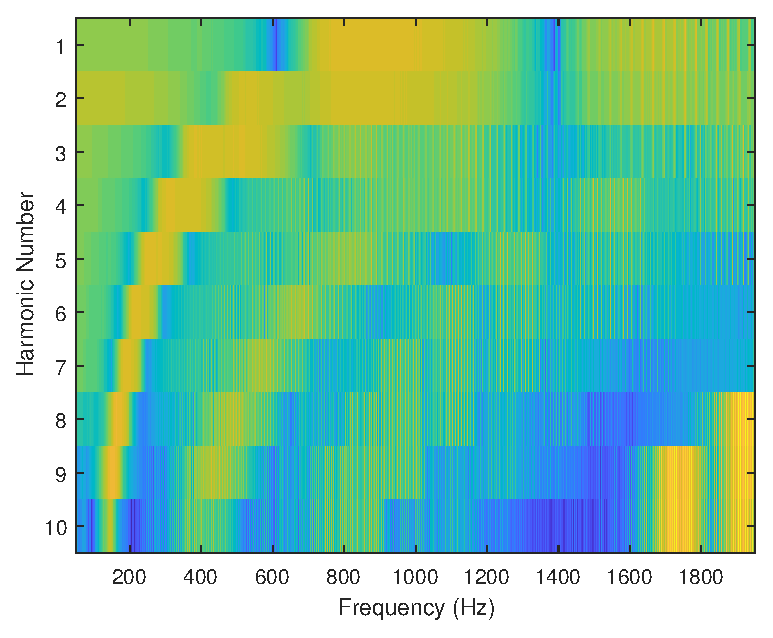
\includegraphics[width=\textwidth]{./dasp_algorithm_results/scap_hasp_filenum_12001.eps}
	\centering
	\caption{SCAP image, $\bf{S}_H$, generated by applying the HASP-D algorithm to the autocovariance vector, $\bf{S}_F$, shown in Figure \ref{fig:scap_xcov_example}.}
	\label{fig:scap_hasp_example}
\end{figure}

Figure \ref{fig:scap_xcov_example} shows a significant number of correlation peaks resulting from the equal spacing of peaks within the frequency spectrum of $\hat{r}$.  The dominant peak occurs at $16$kHz along with corresponding sub-correlations at integer divisions of $16$kHz.  An additional unrelated correlation ``hump'' occurs between $200$Hz and $400$Hz.  Although the previously identified oscillator frequencies from Figure \ref{fig:hasp_fft_example} resulted in significant peaks in the FFT spectrum, the correlation spectrum did not return a strong response, although still identifiable at a much lower level.   This was likely due to the low frequency instability in the signals, identified in Figure \ref{fig:haspd_example_zoom}, as well as the close proximity of the two oscillators resulting in a diminished correlation value.

\section[Cross-Modulation Aligned Signal Projection (CMASP)]{Cross-Modulation Aligned Signal Projection (CMASP)}
\label{Cross-Modulation Aligned Signal Projection}

In addition to carrier frequencies having significant harmonic content, modulation sidebands around a given carrier frequency and its respective harmonics can also have significant harmonic content.  The CMASP algorithm was developed to find the intersection of carrier and modulation frequencies, much like the MASP algorithm, but also provide a mechanism for highlighting the harmonic content of the modulation sidebands, such as the harmonics of $20$Hz previously noted in Figure \ref{fig:masp_example}.  Figure \ref{fig:cmasp_diagram} provides a graphical depiction of the CMASP process as applied to a nominal FFT spectrum.   The CMASP process sweeps across all potential carrier frequencies within a band of interest and provides a sum of the power spectrum of a given carrier frequency and its harmonics, much like the HASP process, but also includes a summation of modulation frequency sidebands and related harmonics.  The CMASP process results in a modulation frequency by carrier frequency image with an ``X'' and associated peaks corresponding to the intersection of a carrier and modulation frequency and their respective harmonics.

\begin{figure}[tp]
	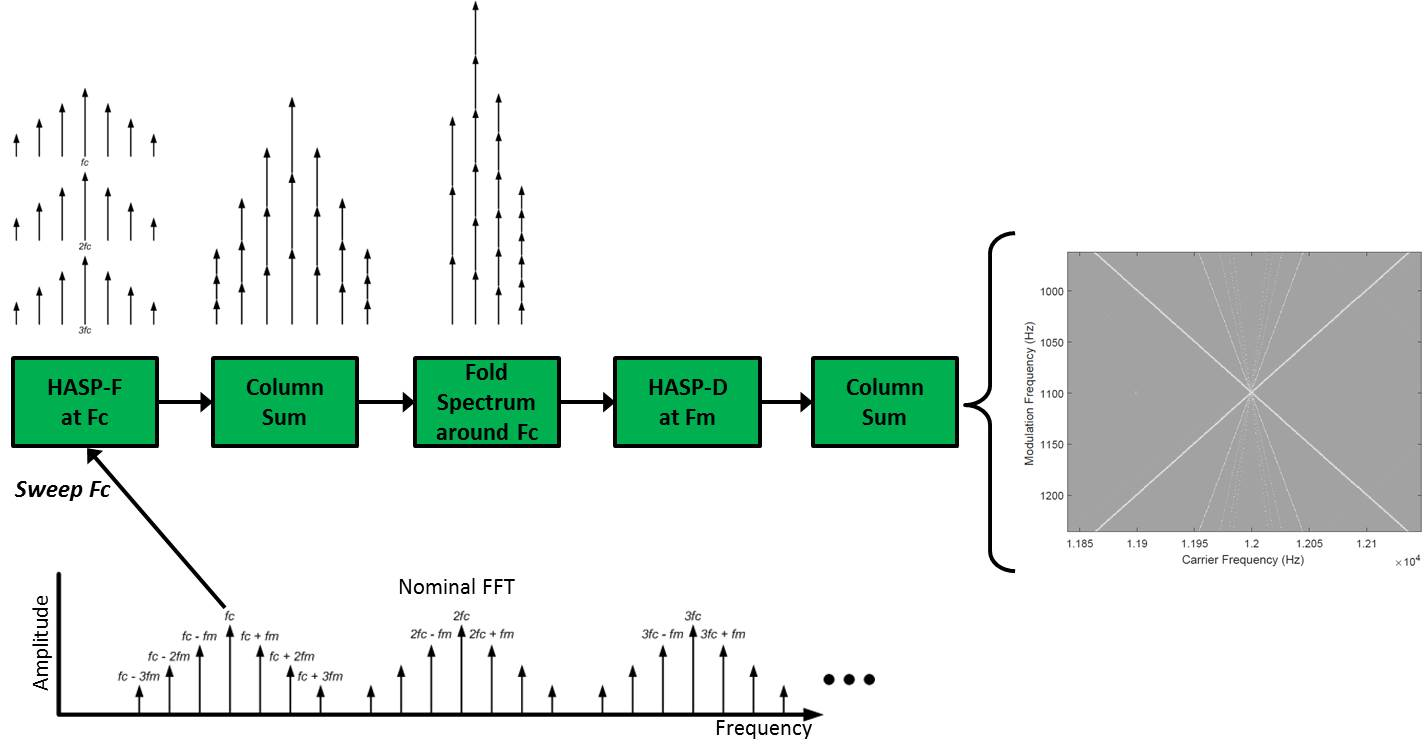
\includegraphics[width=\textwidth]{./misc_graphics/cmasp_diagram.jpg}
	\centering
	\caption{Diagram of the CMASP process as applied to a signal with a carrier frequency ($f_c$) and modulation frequency sidebands ($f_m$), where $f_c$ and $f_m$ both have harmonic content.  The CMASP process sweeps across $f_c$ and aligns the harmonics of the modulation frequency to highlight the intersection of carrier and modulation frequencies.}
	\label{fig:cmasp_diagram}
\end{figure}

The CMASP process is described further in Algorithm \ref{alg:cmaspalg}.  The CMASP process operates on an input signal's power spectral density, $\hat{r}$, and requires carrier center frequency ($f_c$), carrier frequency bandwidth ($B_c$), modulation center frequency ($f_m$), and modulation frequency bandwidth ($B_m$) inputs.  The algorithm initially performs the HASP-F algorithm on $\hat{r}$ and sums all columns in to a 1-D vector.  The 1-D vector is then folded around the center frequency bin and summed to add the lower and upper sideband components.  The HASP-D algorithm is applied to the folded and summed vector to align the harmonics of the modulation frequency.  Finally, the HASP-D output is summed along all columns with the resulting vector forming a single column in the CMASP image.  The process is repeated for all frequency bins within the carrier frequency bandwidth to form a modulation frequency by carrier frequency matrix, with dimensions of $f_m \pm B_m$ by $f_c \pm B_c$, respectively. 

\begin{algorithm}
	\caption{Cross-Modulation Aligned Projection Algorithm} \label{alg:cmaspalg}
	\scriptsize
	\centering
	\begin{algorithmic}[1]
		\Require~~
		\Statex $\hat{r}$ - Input Power Spectrum
		\Statex $f_c$ - Carrier Center Frequency 
		\Statex $f_m$ - Modulation Center Frequency 
		\Statex $B_c$ - Carrier Frequency Bandwidth
		\Statex $B_m$ - Modulation Frequency Bandwidth
		\Ensure~~
		\Statex $\bf{C}$ - CMASP Output Array
		\Statex
		\ForAll  {$i$, where $(k \times f_c) - B/2 \leq f_i \leq (k \times f_c) + B/2$} 
		\State    $\bf{C_m} \gets $ HASP-F($\hat{r}$, $f_i$, $B_c$)
		\State 		$\bf{C_m} \gets $ COLUMN SUM of $\bf{C_m}$
		\State 		$\bf{C_m} \gets \bf{C_m}$(END$/2$ to $1$) + $\bf{C_m}$(END$/2$ to END)
		\State		$\bf{C_m} \gets $ COLUMN SUM of HASP-D($\bf{C_m}$, $f_m$, $B_m$)
		\State		$i$-th column of $\bf{C} \gets \bf{C_m}$
		\EndFor
	\end{algorithmic}
\end{algorithm}

To illustrate the CMASP output, a synthetic signal was generated by amplitude modulating a square wave at a frequency of $12$kHz with a square wave at $1100$Hz.  The resulting power spectral density of the synthetic signal consisted of multiple harmonics of the $12$kHz carrier signal along with multiple upper and lower sidebands comprised of the $1100$Hz modulating frequency and its corresponding harmonics.   Figure \ref{fig:cmasp_synth_example} shows the output of the CMASP process as applied to the synthetic test signal.   The large ``X'' within the image is the result of the intersection of the carrier frequency and the fundamental modulation frequency.  The additional radials at progressively smaller angles are the result of sidebands from the modulation frequency harmonics.  Furthermore, the left-right mirrored radials are due to the presence of both upper and lower modulation sidebands.  Analysis of Figure \ref{fig:cmasp_synth_example} therefore shows a $12$kHz carrier signal being modulated by a $1100$Hz signal with both upper and lower sidebands and multiple harmonics.

\begin{figure}[tp]
	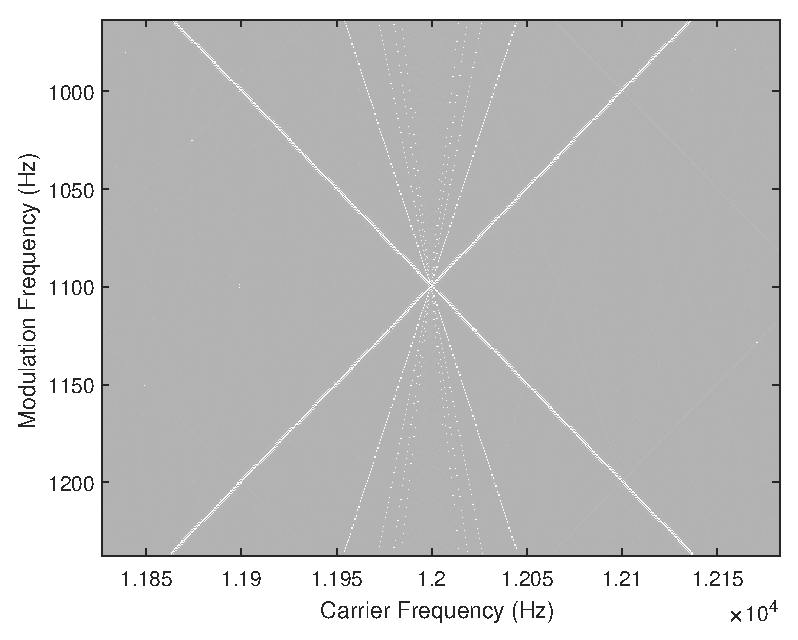
\includegraphics[width=\textwidth]{./dasp_algorithm_results/cmasp_synth.eps}
	\centering
	\caption{CMASP output image resulting from application of the CMASP algorithm to synthetic data.  The synthetic data was generated by multiplying a $1100$Hz square wave with a $12$kHz square wave carrier frequency.  The ``X'' represents the intersection of a modulation frequency at $1100$Hz and its harmonics with a carrier frequency at $12$kHz.}
	\label{fig:cmasp_synth_example}
\end{figure}

Figure \ref{fig:cmasp_example} shows the CMASP algorithm applied to the conducted URE signal from the fluorescent lights as shown in Figure \ref{fig:hasp_fft_example}.  Several radials and intersections are identifiable, with the most prominent occurring at $120$Hz and its respective harmonics.  Single lines appearing with no obvious intersection with a mirrored radial are likely due to unmodulated frequency peaks within the spectrum.
 
\begin{figure}[tp]
	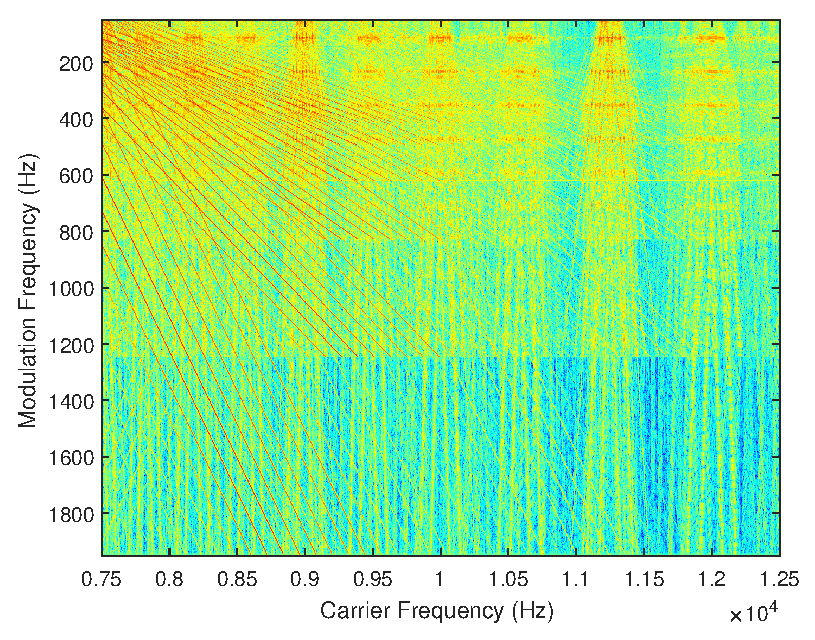
\includegraphics[width=\textwidth]{./dasp_algorithm_results/cmasp_filenum_9601.eps}
	\centering
	\caption{CMASP output image resulting from the fluorescent light conducted URE spectrum shown in Figure \ref{fig:hasp_fft_example}.}
	\label{fig:cmasp_example}
\end{figure}

\section[Frequency Aligned Signal Projection (FASP)]{Frequency Aligned Signal Projection (FASP)}
\label{Frequency Aligned Signal Projection}

The FASP algorithm performs FFTs on short time segments of a time domain signal and aligns the frequency bins of each processed time slice, as detailed in Algorithm \ref{alg:faspalg}.  The FASP algorithm operates on a time domain input signal, $r$, and only requires the number of times slices, $N$, as an input parameter.  Given a fixed length capture, with capture time, $T_c$, and sample rate, $F_s$, the FASP algorithm returns a time by frequency image with dimensions of $\frac{T_c}{N}$ seconds by $\frac{F_s}{2}$Hz.

\begin{algorithm}
	\caption{Frequency Aligned Signal Projection Algorithm} \label{alg:faspalg}
	\scriptsize
	\begin{algorithmic}[1]
		\Require~~
		\Statex $r$ - Input Time Domain Signal
		\Statex $N$ - Number of Time Slices of a Fixed Length Capture File
		\Ensure~~
		\Statex $\mathbf{F}$ - FASP Output Array
		\Statex
		\For  {$n = 1, 2, \ldots N$} 
		\State Row $n$ of $\mathbf{F} \gets $ FFT of $r(x_i)$ where, $(n - 1)T_c/N < x_i < nT_c/N$
		\EndFor
		\State $\mathbf{F} \gets \left|\bf{F}\right|$
	\end{algorithmic}
\end{algorithm}

Figure \ref{fig:fasp_example} shows the FASP algorithm applied to same time domain URE capture represented in Figure \ref{fig:hasp_fft_example}.  As previously noted, the separation of the two fluorescent light $45$kHz oscillator harmonics can be seen at the higher frequencies.   Although not as clear, a slight ``wobble'' on the fundamental frequency and its harmonics can be seen over time resulting from the low frequency modulations identified in Figure \ref{fig:haspd_example_zoom} and Figure \ref{fig:masp_example}.  Given a capture time of one second and a sample rate of $2$MS/s, each row represents a $0.2$ms time slice with the frequency axis spanning $0$ to $1$MHz.
 
\begin{figure}[tp]
	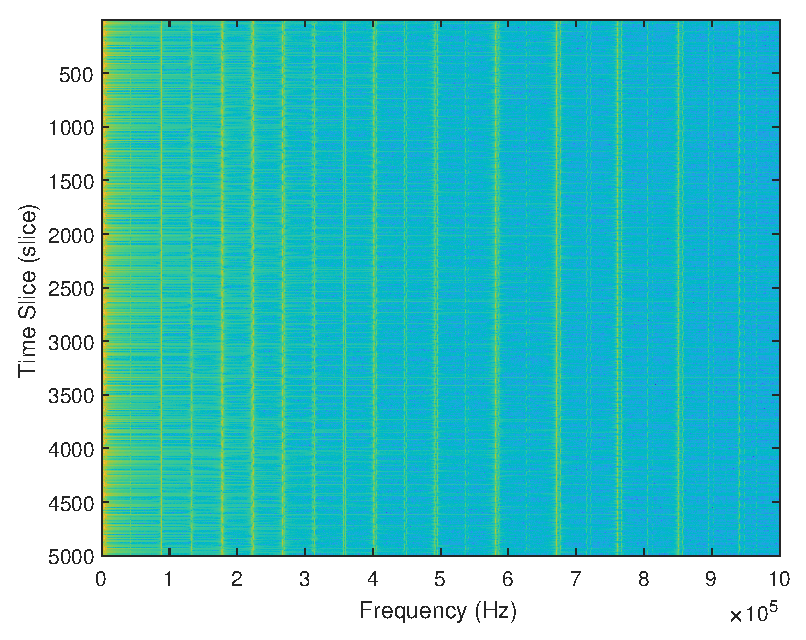
\includegraphics[width=\textwidth]{./dasp_algorithm_results/fasp_filenum_9601.eps}
	\centering
	\caption{FASP algorithm applied to the conducted URE signal illustrated in Figure \ref{fig:hasp_fft_example}.  The $45$kHz carriers and respective harmonics are clearly seen throughout the spectrum on all time slices, with the spacing between their harmonics progressively increasing.}
	\label{fig:fasp_example}
\end{figure}
